\section{Devices}
\label{sec:devices}

We had to build prototypes for research purposes and needed to decide which wearables we intend to work with.
Although we wanted to support the widest range of devices that we could, we had to ditch some in order to be able to iterate fast.
In the following section, we will list the advantages and disadvantages of different wearables.
Namely, we evaluated the Apple Watch, the UP and Microsoft Band as well as Android watches (shown in figure \ref{fig:devices}).

\begin{figure}[H]
	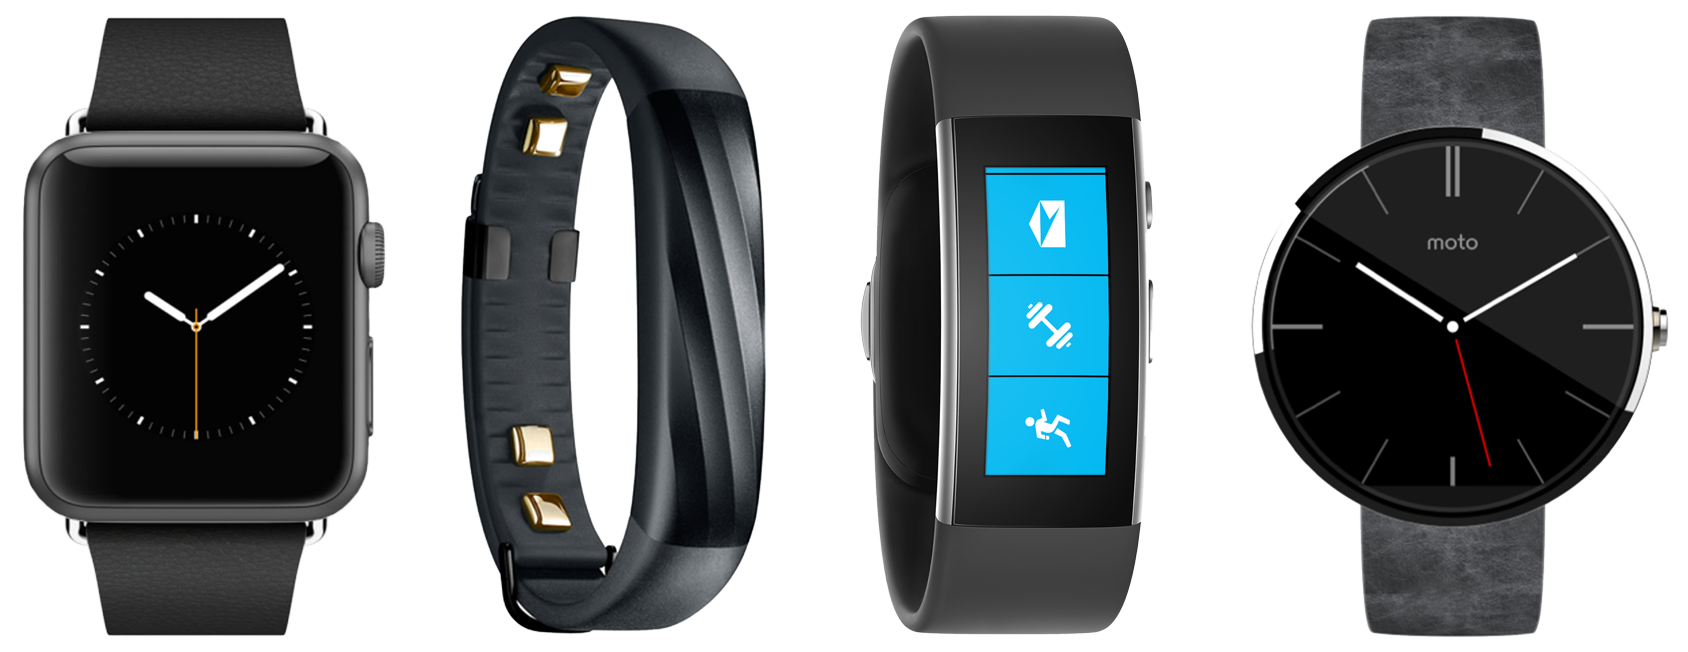
\includegraphics[width=\linewidth]{images/devices.png}
	\caption[Caption for devices]{Wearable devices, in order of appearance}
	\label{fig:devices}
\end{figure}

\subsection{Apple Watch}
While the currently available Apple Watches all provide sufficient hardware and enough sensors, the software does not allow 3rd party developers to take full advantage of this.
With WatchOS 2, Apple restricted apps running on the watch to only get access to sensor data while it's visible to the user.
For our project however, we needed a way to access sensor data from a background service, which simply isn't possible with the existing APIs.
Apple announced that in WatchOS 3 (which isn't available yet), this restriction will be eliminated. 

\subsection{UP by Jawbone}
Jawbone's fitness trackers follow an approach that differs from the other wearables.
Raw data from the few built in sensors is stored on the device.
It occasionally synchronizes this data with the ``UP'' app for iOS and Android via Bluetooth, which then uploads the data to Jawbone's servers.
The servers process the raw data and extract useful information, which is then accessible through an API.
This results in an delay of about 2 hours, which means that we can not use it in any real-time related context.
Even if that delay would be acceptable, the API does not provide access to the raw sensor data, which would be required for our project.

\subsection{Microsoft Band}
Although Microsoft also decided to synchronize raw data from the device sensors to their own ``Microsoft Health'' app, they don't need to send it to their servers in order to process it.
Developers can integrate an SDK into their applications, which allows them to subscribe to sensors available on the device.
Unfortunately the sampling rate is limited to the SDK capabilities and does not leave room for custom implementations.

\clearpage

\subsection{Android Wear}
Android Wear is a platform for smartwatches that many devices from different manufacturers build upon.
Although it is customized to match the conditions of a watch, it still is a full Android OS without any limitations.
Because of Androids open nature, it is possible to deploy custom apps and to use everything that the devices offer without any software restrictions.
All currently available devices powered by Android Wear have the sensors that we needed for our project built in.

\subsection{Decision}

The fitness trackers by Jawbone do not provide access to the raw sensor data in real-time.
Even though they feature great hardware, the software lacks functionality and renders the devices unusable for us.

Microsoft Bands would be possible candidates for our project, but they don't offer a lot of customizability.
In addition to that, they have a much smaller user base compared to the wearables by other manufacturers.

Unlike the Apple Watch, Android Wear devices are able to connect to devices that don't belong to the same ecosystem, which increases the number of potential users. Although Apple topped Androids market share by almost 30\%\footnote{According to IDC Worldwide Quarterly Wearable Device Tracker} in 2015, we decided to develop for the Android platform because of the restrictions of WatchOS 2 mentioned above.

\clearpage